\documentclass[tikz,crop]{standalone}

\usepackage{tikz,pgfplots}

\usetikzlibrary{decorations.shapes}
\usetikzlibrary{arrows.meta,calc,decorations.markings,math,arrows.meta}


%%%%%%%%%%%%Todo está en 2D porque no entiendo 3D   :c


\begin{document}
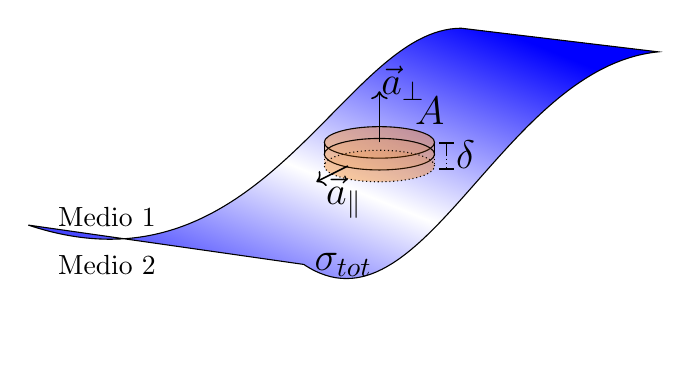
\begin{tikzpicture}%[scale=1.5]
%\draw (3.46,1.9) circle(2pt);ESTA ES LAREFERENCIA PARA ANTES DE MOVER LAS COSAS

%%%%%%%%%%%%%%%%%%%%%%%%%%%%%%%%%%%%%%%%%%%%%%%% 	SUPERFICIE
\shadedraw[	top color =blue,				%%%%	Color de arriba
			bottom color =blue,				%%%%	Color de abajo
			middle color = white, 			%%	Color de en medio
			shading angle = -22]			%%%%	Ángulo de gradiente
			
(-1,1) ..controls (2, 0) and (3,3.5) .. (4.5,3.5) %	Aquí se dan las lineas
-- (7,3.2) .. controls (5,3) and (4,-.5) .. (2.5,.5)%	A .. ctrls P and Q.. B 
--(-1,1);								%%%%%%%%%	P y Q jalan la linea de A a B
\node[color = black] at (3,.5) {\Large $\sigma_{tot}$};
\node  at (0,1.1) {Medio 1};
\node at (0,.5) {Medio 2};



%%%%%%%%%%%%%%%%%%%%%%%%%%%%%%%%%%%%%%%%%%%%%%%%%%%%%%%%%	PILL-BOX
\fill[orange, opacity = .3]						%%%%%%%%	Cara del cilindro
 (3.46-.7,2.05) arc(180: 0: .7 and .2)			%%%%%%%% 	se pone el principio pero es
-- (3.46+.7,1.75) arc(0: -180: .7 and .2)		%%%%%%%		lo ultimo que puedo escribir
-- (3.46-.7,2.05);

\draw[black](3.46,2.05) circle (.7 and .2)		%%%%%%		Centro y radios de curvatura
(4.1,2.15)node[above]{\Large $A$};	%%%%		Etiqueta del área
\fill[orange, opacity = .1] (3.46,2.05) circle (.7 and .2); 

\draw[black](3.46,1.9)  circle (.7 and .2);
\fill[orange,opacity = .1](3.46,1.9)  circle (.7 and .2);

\draw[densely dotted, black](3.46,1.75)  circle (.7 and .2);
\fill[orange,opacity = .1](3.46,1.75)  circle (.7 and .2);

\draw[black, line width = .2mm]						%%%%%%	Lineas que faltó llenar
(3.46-.7,2.05) -- (3.46-.7,1.9)		(3.46+.7,2.05) -- (3.46+.7,1.9);
\draw[densely dotted, black, line width = .2mm]
(3.46-.7,1.9) -- (3.46-.7,1.75)		(3.46+.7,1.9) -- (3.46+.7,1.75);
 
 
 
  
%%%%%%%%%%%%%%%%%%%%%%%%%%%%%%%%%%%%%%%%%%%%%%%%%%%%%%%%%%%%	VECTOR NORMAL (Perp)
\draw[ -> ,line width=.2mm, black]	
 (3.46,2.05)--(3.46,2.6+.1);	%%%%	Se toma un punto medio y se desplaza para dar profundidad
\node[color = black, right] at (3.46-.1,2.6+.2) {\Large $\vec{a}_\perp$};%	Se etiqueta la flecha

%%%%%%%%%%%%%%%%%%%%%%%%%%%%%%%%%%%%%%%%%%%%%%%%%%%%%%%%%%%%	VECTOR NORMAL (Paralelo)
\draw[-> ,line width=.2mm, black]	
 (3.46-.7+.3, 1.9-.15)-- (3.46-.7-.1,1.95-.4);	
\node[color = black, left] at (3.46-.1,1.95-.6) {\Large $\vec{a}_\parallel$};%	Se etiqueta la flecha




%%%%%%%%%%%%%%%%%%%%%%%%%%%%%%%%%%%%%%%%%%%%%%%%%%%%%%%%%	LINEA DE ALTURA
\draw[|-, line width=.2mm,black]
(3.46+.7+.15,2.05) -- (3.46+.7+.15, 1.9);
\draw[-|, densely dotted, line width=.2mm,black]
(3.46+.7+.15,1.9) -- (3.46+.7+.15,1.7);
\node[color = black, right] at (3.46+.7+.15,1.9) {\Large $\delta$};









\end{tikzpicture}
\end{document}